\documentclass[oneside]{book}

\setcounter{tocdepth}{1}
\setcounter{secnumdepth}{3}

\usepackage[toc,page]{appendix}
\usepackage{hyperref}
\usepackage[utf8]{inputenc}
\usepackage{graphicx} % Required for the inclusion of images
\usepackage{amsmath} % Required for some math elements 
\usepackage[utf8]{inputenc}
\usepackage[english]{babel}
\newtheorem{theorem}{Theorem}
\newtheorem{corollary}{Corollary}[theorem]
\newtheorem{lemma}[theorem]{Lemma}
\usepackage{listings}
\usepackage{pdfpages}
\usepackage{amssymb}
\usepackage{pdflscape}

\begin{document}

\begin{titlepage}
	\centering
	
\includegraphics[width=0.60\textwidth]{../../logo/UoN_Primary_Logo_RGB.png}\par\vspace{1cm}
	\vspace{1.5cm}
	{\huge\bfseries Comparing the Pure Functional and Object Oriented Paradigm for implementing ABS \par}
	\vspace{2cm}
	{\Large\itshape jonathan.thaler@nottingham.ac.uk \par}
	\vfill
	
	\vfill

	{\large \today\par}
\end{titlepage}

\cleardoublepage

\section*{Abstract}
This study we compares the object oriented and pure functional programming paradigms to implement Agent-Based Simulation. Due to fundamentally different concepts both propagate fundamental different approaches in implementing ABS. In this document we seek to precicesly identify these fundamental differences, compare them and also look into general benefits and drawbacks of each approach.

\clearpage
\tableofcontents
\clearpage

\section{Introduction}
There exists a large number of simulation packages which allow the convenient creation of System Dynamics simulations by straight-forward visual diagram creation. One simply creates stocks and flows, connects them, specifies the flow-rates and initial parameters and then runs the model. An example for such a visual diagram creation in the simulation package AnyLogic can be seen in Figure \ref{fig:sir_stockflow_diagram}.

\begin{figure}
	\centering
	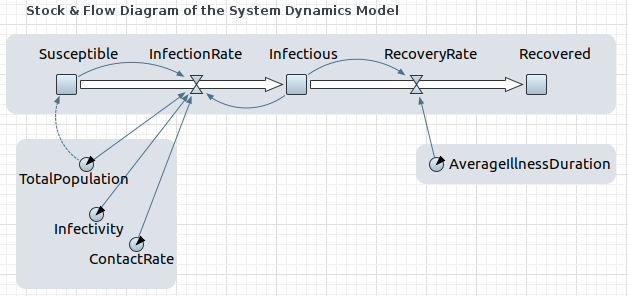
\includegraphics[width=.5\textwidth, angle=0]{./fig/SIR_SD_STOCKFLOW_DIAGRAMM.png}
	\caption{Visual System Dynamics Diagram of the SIR model in AnyLogic Personal Learning Edition 8.3.1.}
	\label{fig:sir_stockflow_diagram}
\end{figure}

Still, implementing System Dynamics directly in code is not as straight forward and involves numerical integration which can be quite tricky to get right. Thus, the aim of this paper is to look into how System Dynamics models can be implemented in code correctly without the use of a simulation package. We use the well known SIR model \cite{kermack_contribution_1927} from epidemiology to demonstrate our approach.

Our language of choice is Haskell because it emphasises a declarative programming style in which one describes \textit{what} instead of \textit{how} to compute. Further it allows to rule out interference with non-deterministic influences or side-effects already at compile-time. This is of fundamental importance for System Dynamics because it behaves completely deterministic and involves no stochastics or non-determinism whatsoever. Also, we make use of Functional Reactive Programming which allows to express continuous-time systems in a functional way. 

We show that by this approach we can arrive at correct-by-construction implementations of System Dynamic models. This means that the correctness of the code is obvious because we have closed the gap between the model specification and its implementation. Thus, the contribution of the paper is the demonstration of how to implement correct-by-construction System Dynamics simulations using Haskell and Functional Reactive Programming.

\chapter{Challenges}

The challenges one faces when implementing an Agent-Based Simulation (ABS) plain, without support from a library (e.g. Repast) are manifold. In the paper on update-strategies (TODO: cite) we've discussed already in a very general, programming language agnostic way, the fundamental things to consider. Here we will look at the problem in a much more technical way by precisely defining what problems need to be solved and what approaches are from a programming paradigm view-point - where we focus on the pure functional (FP) and imperative object-oriented (OO) paradigms.

Generally one faces the following challenges:

\begin{enumerate}
	\item Agent Representation - How is an Agent represented in the paradigm?
	\item Agent Updating - How is the set of Agents organized and how are all of them updated?
	\item Agent-Agent Interactions 
	\item Environment Representation
	\item Environment Updating
	\item Agent-Environment Interactions
	\item Replications
\end{enumerate}

It is important to note that we are facing a non-trivial software-engineering problem which implies that there are no binary correct \ wrong approaches - whatever works good enough is OK. This implies that the challenges as discussed below, can be also approached in different ways but we tried to stick as close as possible to the \textit{best practices} of the respective paradigm.

\section{Agent Representation}
\subsection{OO}
In the OO paradigm an Agent will (almost) always be represented as an object which encapsulates the state of the Agent and implements the behaviour of the Agent into private and public methods. Care must be taken to not confuse the concept of an Agent with the one of an object: an Agent is pro-active and always in full control over its state and the messages sent to it. We have discussed pro-activity in the update-strategies paper already: what is needed is a method to update the Agent which transports some time-delta to allow the Agent perceive time, ultimately allowing it to become pro-active. Other options would be to spawn a thread within the object which then makes the object an \textit{active} object but then one needs to deal with synchronization issues in case of Agent-Agent interactions. 
In OO it is tempting to generate getter and setter for all properties of the Agent state but this would make the Agent vulnerable to changes out of its control - state-changes should always come from the Agent within. Of course when generating text- or visual output then getter are required for the properties which need to be observed.
Agent-creation in OO is then in the end an instantiation of an Agent-Class resulting in an Agent-Object. When one strictly avoids setter-methods then the only way of instantiating the Agent into a consistent state is the constructor. This could lead to a very bloated constructor in the case of a complex Agent with many properties. Still we think this is better than having setter-methods as setters are always tempting to be used outside of the construction phase, especially when multiple persons are working on the implementation or when the original implementer is not available any more. If an Agent construction is really complicated with many constructor-parameters one can resort to the Builder-Pattern \cite{bloch_effective_2014}. Another approach to creation is dependency injection \footnote{See \url{https://martinfowler.com/articles/injection.html}} but then the application would need to run in an IoC container e.g. Spring. We haven't tried this approach but we think it would over-complicate things and is an overkill in the domain of ABS. TODO: add some illustrating code

\subsection{FP}
Although there exist object-oriented approaches to functional programming (e.g. F\#, OCaml) we assume that there are no classes and inheritance in FP. By a class we understand a collection of functions (called methods in OO) and data (members or properties in OO) where the functions can access this data without the need to explicitly pass it in through arguments.
So we need functions which represent the Agent's behaviour and data which represents the Agents state. The functions need to access this state somehow and be able to change the state. This may seem to be an attempt to emulate OO in FP but this is not the case: functions operating on data are not an OO-exclusive concept - it becomes OO when the data is implicitly bound in the function \footnote{We are aware that OO is characterized by many more features e.g. inheritance, but we don't go into those details here as they are not relevant anyway - we simply want to show the subtle differences in Agent-representation of FP and OO where it suffices to emphasise the concept of implicitly / explicitly bound data}.
FP in general has no notion of a compound data-type but tuples can be used to emulate such. Because it is quite cumbersome to work on tuples or to emulate compound data-types using tuples, FP languages (e.g. Haskell) have built-in features for compound data-types. So we assume that without loss of generality (because compound data-types are in the end tuples with different names for projection-functions) Agent state in FP is represented using a compound data-type.
The relevant function in FP for Agent-Behaviour is the update-function. We have two options:
Either the function arguments are the compound agent-state, time-delta and incoming messages and must return the (changed) compound agent-state and outgoing messages.
Or we use continuation-style programming in which the compound agent-state is updated internally and the only input are the time-delta and incoming messages and the output are outgoing messages, the observable agent-state which can be represented by a different compound data-type AND a continuation function.
In the first approach the full agent-state is available outside and could be changed any time - there is no such thing as data-hiding in this case. In the continuation case the state is bound in a closure which is the newly constructed function which will be returned as continuation. This is only possible in a real functional language which allows the construction of functions through lambdas AND return them as a return value of a function. TODO: add some illustrating code

\section{Agent Updating}
\subsection{OO}
After creating the Agents one ends up with a collection of Agents, represented either as a List, a Vector or a Map. In OO updating is pretty trivial: one iterates over the collection and calls some update-method of the Agent objects. This implies that if one uses inheritance and has a general Agent-Class, this class needs to provide an update-method which feeds a time-delta.
When implementing the parallel-strategy things become complicated in OO though. Changes must only be visible in the next iteration. This can only be achieved by either messaging instead of method-calls or creating new Agent-objects after every iteration.

\subsection{FP}
In FP after the construction phase one also ends up with a collection of Agents either a list or a Map. Updating in FP is more subtle because it lacks references and mutable data. In case of the sequential strategy more work needs to be done and we can see the problem in general as a fold over the list of agents. In the case of the parallel strategy we can directly make use of FPs immutability.

\section{Agent-Agent Interactions}
\subsection{OO}
In OO we have basically two possibilities to implement Agent-Agent Interactions: either by direct method calls to the other Agent which requires the calling Agent to hold a reference \textit{with the subtype of the callee if using an abstract Agent-Class} OR by adding messages to a message-box (e.g. a HashMap or List) of the receiving Agent. Both have fundamental differences: a direct method call is like transferring the action to the callee: the Agent suddenly becomes active where before the calling Agent was active - as soon as the callee has finished the method, action returns to the callee. Note that the callee can again call other Agents methods which could, if not guarded explicitly against, lead to a cycle if the model-semantics permit it.
When adding a message to a message-box no action is transferred to another Agent. Still a reference to the Agent with type of the abstract Agent-Class must be held if one implements it as a direct access to the mailbox. This has the advantage that it is fast but the disadvantage that we deal again with references and need synchronization in case of parallelism/concurrency. Another option would be to have a outgoing-box into which the Agent adds messages it wants to send and the ABS system handles then the delivery after each step. This has the advantage that no direct references to other Agents are required, only their (numerical) IDs but the disadvantage that this delivery process has O($n^2$) complexity (TODO: prove that or back it up with evidence. could we also reduce it to O (n log n) when using a map? or is it even possible to somehow use O (n)?)
\subsection{FP}
In FP when staying completely pure the only option we have is an outgoing-box into which messages are queued and the ABS system then distributes them into the ingoing-boxes of the receivers. This is because we have no method calls - of course we could simulate method calls by dragging the complete state around which would allow to execute some message-handler by the receiving Agent within the calling Agent but then the Agents themselves need to be aware of implementation-details and have full access to all other agents - reasoning becomes difficult and robustness will inevitably suffer, so we won't go there.
If we allow explicit side-effects in the form of Monadic programming then we can implement direct access to other Agents mailboxes as in the OO version: either we use references and run in the IO monad or we use STM channels and run in the STM monad. As IO would ruin very much we can reason about the most reasonable approach would be to make use of STM. But as long as there is no real need for concurrency as in the concurrent- and actor-strategies STM is an overkill and we will stick to outgoing boxes. This buys us the reasoning abilities and robustness but hits us with a penalty in performance.

\section{Environment Representation}
\subsection{OO}
An Environment can be represented quite arbitrarily in OO and shared between the Agents using references. The downside is that it must be protected in case of parallel or concurrent access.
\subsection{FP}
Here we can go again two ways: stay pure or use explicit side-effects using IO or STM references. When staying pure the environment must be passed in through the behaviour function - and returned if it has changed. This allows us to easily reason which functions only read the environment, change it or don't need it at all: its visible from the type of the function and we can guarantee it statically at compile-time.
Things are not so when using references (either STM or IO) as reading or writing both requires to run in the Monad thus making it not possible any more to tell at compile-time and rather from the type if its a read or write operation - we can only tell that the environment is touched or not. Also the behaviour-function must run in the respective monad although the environment is never accessed, thus removing further abilities to reason.

\section{Environment Updating}
\subsection{OO}
The ABS system holds a reference to the Environment which will be accessed and changed by the Agents through references. The Environment class can implement some update-function which can then be called by the ABS system in every step, allowing the environment to update itself (e.g. regrowing some resource)
\subsection{FP}
In the FP version the ABS holds also an instance of an environment data-structure and if the environment should be able to update itself (e.g. regrowing some resource) then simply a environment-behaviour function must be provided which just maps the environment-type to the environment-type and has some time-input: (Double -> e -> e)

\section{Agent-Environment Interactions}
\subsection{OO}
Agents simply call methods on the Environment to which they hold a reference thus changing the environment. The problem is much more subtle if we want true parallel or concurrent / actor strategies. In the case of parallel strategy the other agents must not see the changes to the environment. In the case of the concurrent / actor strategies the access to the environment must be synchronized.
\subsection{FP}

\section{Replications}
\subsection{OO}
Replications need careful considerations in OO especially when using global references and data \textit{when running them in parallel \footnote{If not then one does not need to care further}}. All objects which have mutable state need to be accessed only by one replication thus one might to change the implementation to allow parallel replication.
\subsection{FP}
In FP running Replications in parallel or not makes to difference from a programming perspective: because of the nature of FP we can execute multiple simulations in parallel. Of course copying the initial agents and environment is necessary but that is very easily done in FP.

\renewcommand\bibname{References}

\bibliographystyle{acm}
\bibliography{../../references/phdReferences}

\end{document}
